% ----------
% A LaTeX template for course project reports
% 
% This template is modified from "Tech Report ala MIT AI Lab (1981)"
% 
% ----------
\documentclass[12pt, letterpaper, twoside]{article}
\usepackage{geometry}
\usepackage[utf8]{inputenc}
\usepackage[english]{babel}
\usepackage[runin]{abstract}
\usepackage{titling}
\usepackage{booktabs}
\usepackage{fancyhdr}
\usepackage{helvet}
\usepackage{csquotes}
\usepackage{graphicx}
\usepackage{parskip}
\usepackage{etoolbox}


\input{preamble.tex}

% ----------
% Variables
% ----------

\title{\textbf{Cybersecurity Course Project:\\Deception database generator}} % Full title of your tech report
\runningtitle{Deception database generator} % Short title
\author{Daniele Santini} % Full list of authors
\runningauthor{Daniele Santini}
\affiliation{Alma Mater Studiorum - Università di Bologna} % Affiliation e.g. University or Company
\department{} % Department or Office
\memoid{Project 2} % Project group ID that were shared with the class earlier.
\theyear{2023} % year of the tech report
\mydate{December 14, 2023} %the date


% ----------
% actual document
% ----------
\begin{document}
\maketitle

\begin{abstract}
    \noindent
    
    By creating fake services and components that appear as valuable targets to attackers, defenders can divert the attacker's attention and resources away from critical assets. Attackers might spend time and effort trying to compromise these fake elements, leaving less capacity to target actual valuable assets.
    In this project I explore the implementation of a fake relational Database generator, leveraging open source generative AI for content generation.

    % Uncomment the following to add keywords as needed
    % \keywords{Keyword1, Keyword2, Keyword3}
\end{abstract}

\vspace{2.5cm}

% Uncomment the following to add thanks.
% {\footnotesize
%     \noindent
%     Special thanks to \textbf{Person 1} and \textbf{Affiliation A} for financial support for this project.
% }

\thispagestyle{firstpage}

\pagebreak

% ----------
% End of first page
% ----------

\newgeometry{} % Redefine geometries (normal margins)

\section{Introduction}
\label{sec:intro}

Cybersecurity experts have recently proposed using defensive deception as a means to leverage the information asymmetry typically enjoyed by attackers as a tool for defenders.

By creating fake services and components that appear as valuable targets to attackers, defenders can divert the attacker's attention and resources away from critical assets. Attackers might spend time and effort trying to compromise these fake elements, leaving less capacity to target actual valuable assets.

The goal of this project is to create a tool able to generate fake relational databases pre-packaged in an OCI compatible container images ready to be instantiated and function out of the box. The container image must include all the relevant "fake" data for its correct operation. Eventual configuration have to be provided during the generation to build the final working image.

The DB has to be able to import an existing schema or generate a new one and then generate data to populate it, providing configurable settings for client connections (port, authentication, credentials).

\section{Discovery}
\label{sec:discovery}

OCI is the leading specification for container images. Multiple toolchains exist for generating OCI compatible images. A non comprehensive list includes:
\begin{itemize}
    \item \verb|docker build| (part of the Docker suite, builds images from Dockerfiles)
    \item \verb|buildah| (builds images from shell scripts)
    \item \verb|orca-build| (builds images from Dockerfiles or Orcafiles
\end{itemize}
Among these, Docker is the most popular and has the most widespread documentation.

Container runtimes and orchestrators compatible with OCI images include
\begin{itemize}
    \item Kubernetes
    \item Podman
    \item Apache Mesos
    \item Amazon Elastic Container Service (ECS)
    \item Docker Compose and Docker Swarm
\end{itemize}
In the enterprise world Kubernetes is by far the most popular and part of managed offerings by enterprise solution vendors cloud platforms. For very basic needs, tools like Docker Compose offer an easy to use and low-resource alternative.

At this time most Database Management System vendors offer OCI base images for their products. Limiting to relational database vendors, these include
\begin{itemize}
    \item Oracle
    \item PostgreSQL
    \item MySQL
    \item Microsoft SQL Server
\end{itemize}
Most images accept on the first launch environment variables to initialize many configurations (user, password, database name) and in some cases initialization scripts that are run on startup.
For example, in the case of PostgreSQL, the Docker image postgres accepts the following optional configurations on the first container startup:
\begin{itemize}
    \item \verb|POSTGRES_USER| environment variable: sets the initial user name
    \item \verb|POSTGRES_PASSWORD| environment variable: sets the initial user password
    \item \verb|POSTGRES_PASSWORD_FILE| environment variable: like the above, but instead of passing directly the password it specifies the file where the password is located (typically a file mounted through Docker secrets)
    \item \verb|POSTGRES_DB| environment variable: sets the initial database name
    \item \verb|PGDATA| environment variable: sets the folder where the DB data is stored (default: \verb|/var/lib/postgresql/data|)
    \item \verb|/docker-entrypoint-initdb.d| folder: any *.sql, *.sql.gz, or *.sh script located in this folder will be executed on the first startup, allowing to bundle initialization data and/or behaviors
    \item \verb|POSTGRES_INITDB_ARGS| environment variable, sets the argument to pass to the initialization shell script
\end{itemize}

Multiple SaaS platforms exist to generate synthetic data, typically for testing purposes. Some of them include:
\begin{itemize}
    \item Mockaroo: Available as web interface and API, available also as a Docker image for self-hosting but requires a license anyway
    \item Cobbl.io: Available as a web interface
    \item generatedata.com: Available as a web interface, FOSS (GPL3)
    \item Tonic: enterprise oriented, designed to mimic existing production data
    \item Broadcom Test Data Management: enterprise oriented, suite of tools to generate and manage test data
    \item Datprof privacy: enterprise oriented, suite of tools to mask sensitive data from existing production data, generate and manage test data
\end{itemize}

Given the scope of this project, local generative AI, like Large Language Models that can be used directly without requiring access to a third party API, deserve some interest. The most popular locally deployable open source LLMs include:
\begin{itemize}
    \item Llama 2 by Meta
    \item Bloom
    \item Falcon
    \item XGen by Salesforce
\end{itemize}

\section{Design}
\label{sec:design}

Due to its ease of use, widespread documentation and support I choose Docker as image build tool and container runtime, using docker compose to document my development architecture and facilitate the usage of low level docker commands. For the build of the final image I use Docker buildx, which allows to build in one shot the image for multiple architectures.

Regardless of the build toolchain, the output image, being OCI compatible, will be usable by all container orchestrators mentioned above

I choose PostgreSQL as DB type because of the advanced ability to customize it.
As base image I choose \verb|postgres| from Docker Hub, available for both amd64 and arm64.
The version of PostgreSQL can be choosen with the \verb|POSTGRES_VERSION| environment variable.

The latest version is 16 but I choose as default the version 11.2 because it's the latest version to be affected by two high severity CVE registered vulnerabilities (\verb|CVE-2019-9193| and \verb|CVE-2019-10164|), which might attract the attackers more than a newer version without high severity vulnerabilities.

For the schema generation and data generation phases I decided to experiment directly with local generative AI models, in particular I experimented with Llama2 7 billion and 13 billion parameter models.

\section{Implementation}
\label{sec:implementation}

The flow I designed and implemented is represented in Figure \ref{fig:diagram}.

The user can pass a custom schema or generate one using the python script create-schema.py with a description of what needs to be represented as a first argument. However it's worth noting that it's not rare for the model to hallucinate or generate invalid syntax, so the  scripts generates one table at a time with many output files with alternative responses and then the user must always manually check the best correct alternative and copy it into schema.sql.

Then the user can use the ready-to-use bash scripts from this project to build the base image, fill it with generated data and build the full image, which will retain all the customization options cited above from the \verb|postgres| image.

Data generation is based on Llama.cpp, a lighter, more portable alternative to the original Llama model that can use the same weights of the official model. Inside create-initdb.py, which handles this interaction, many requests for data are made to Llama, passing JSON Array as requested response grammar, then for each response the script connects to the DB and tries to connect to the DB and insert it, checking this way if the data was acceptable for the table constraints.

One of the advantages of containers is that they allow to decouple many aspects of the application from the underlying system. Unfortunately one thing that is not decoupled is architecture: images are made for a specific architecture and, for example, arm64 images can be instantiated only on arm64 systems. In the final image build script I configured and enabled Docker buildx, which generates multi-architecture versions of the image for amd64 and arm64 (adding new architectures would just require adding a new line in docker-compose.yaml).

The base image has a default image name but the final image intentionally has no default name and when using this project in production it is extremely important to use realistic names for the generated image in the context where it will be used. Under the right circumstances an attacker can see the name of the image used for a live DB so having a fixed clear name would make the life of attackers really easy in finding the fake DBs.

\begin{figure}
    \centering
    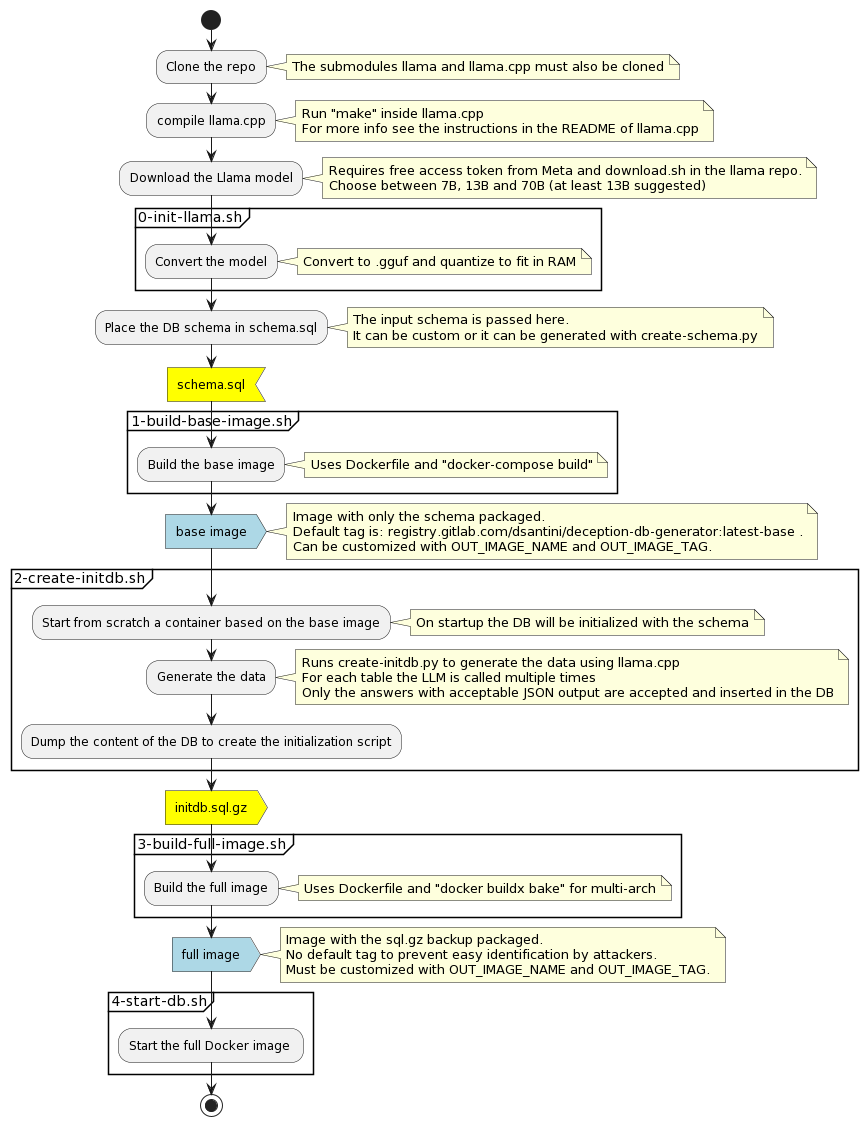
\includegraphics[width=0.9\linewidth]{diagram.png}
    \caption{Diagram of the implementation}
    \label{fig:diagram}
\end{figure}

\section{Conclusions}
\label{sec:conc}

The scripts successfully handles the generation of the DB.

Assuming the right amount of time and compute power is given to the data generation process, the image can be easily used for the original objective of this project.

Llama 7B and 13B model struggle a lot with JSON output despite Llama.cpp built-in grammar support, even after a lot of prompt engineering. This forces the script to repeat generation many times and discard the (many) bad results, inserting the right ones.
For computing power limitations it wasn't possible to use the Llama 70B model and other LLMs, but it would be certainly insightful to test them in this context.


% Uncomment following to add an acknowledgement section
% \section*{Acknowledgements}

% Thanks again to \textbf{Person 1} and \textbf{Affiliation A} for their financial support.

% ----------
% Bibliography
% ----------

% Uncomment the following and add your references into biblio.bib file
% \bibliography{./biblio.bib}
% \bibliographystyle{abbrv}

\appendix

%\section{An appendix}


\end{document}

% ----------
